\documentclass{beamer}
 
\usepackage[utf8]{inputenc}
\usepackage{etoolbox}
\setbeamercovered{transparent}

\usepackage{lmodern}
\usepackage{tikz}
\usetikzlibrary{positioning}
\usetikzlibrary{arrows}
\usetikzlibrary{shapes}

\tikzset{
  treenode/.style = {shape=rectangle, rounded corners,
                     draw, align=center,
                     top color=white, bottom color=blue!20},
  root/.style     = {treenode, font=\Large, bottom color=green!30},
  env/.style      = {treenode, font=\ttfamily\normalsize},
  dummy/.style    = {circle,draw}
  invisible/.style={opacity=0},
  visible on/.style={alt={#1{}{invisible}}},
  alt/.code args={<#1>#2#3}{%
      \alt<#1>{\pgfkeysalso{#2}}{\pgfkeysalso{#3}} % \pgfkeysalso doesn't change the path
  },
}

% \usetheme{Copenhagen}
\usetheme{EastLansing}
\usecolortheme{dolphin}
 
 
%Information to be included in the title page:

\titlegraphic{%
    \vspace*{10mm}
    \makebox[0.9\paperwidth]{%
        \raggedleft\includegraphics[height=1.1cm,keepaspectratio]{pics/oeaw-logo.jpg}%
        \hfill%
        % \hspace*{-10mm}
        \raggedright\includegraphics[height=1.1cm,keepaspectratio]{pics/smi-logo.jpg}%
        % \hspace*{3mm}
    }%
}

\title[Introduction to Machine learning] %optional
{Machine learning methods applied to the analysis of central exclusive production events in ALICE}
 
% \subtitle{A short story}
  
\author[Ratzenböck] % (optional, for multiple authors)
{Sebastian Ratzenböck\inst{1}}

\institute[SMI] % (optional)
{
\inst{1}%
Stefan Meyer Institut\\
Österreichische Akademie der Wissenschaften
}
  
\date[26.April 2018] % (optional)
{26. April 2018}
 
\begin{document}

%------------------------------------------------ 
\frame{\titlepage}

%------------------------------------------------ 

\begin{frame}
    \frametitle{Outline}
    \tableofcontents
\end{frame}

%------------------------------------------------ 
\section{ML: an overview} %

\begin{frame}
    \frametitle{ML: an overview}
    In general ML represents a contrast to a \emph{rule based systems}
    \begin{block}{Rule-based system}
        System that uses rules to make deductions or choices
        \begin{itemize}
            \item<1-> Domain-specific expert system
            \item<2-> Knowledge base: facts \& rules (if $\to$ then statement)
            \item<3-> Rules manually specified (by expert) $\to$ expensive, incomplete
        \end{itemize}
    \end{block}
\end{frame}

%------------------------------------------------ 

% \begin{frame}
%     \frametitle{ML: an overview}
%     In general ML represents a contrast to a \emph{rule based systems}
%     \begin{block}{Machine learning}
%         \begin{itemize}
%             \item<1-> Alorithms that learn from \emph{data} \& make predictions on \emph{data}
%             \item<2-> Automatic methods (no human needed)
%             \item<3-> Human work required for defining problem \& assessing the data
%         \end{itemize}
%     \end{block}
% \end{frame}

%------------------------------------------------ 

\begin{frame}
    \frametitle{ML: an overview}
    In general ML represents a contrast to a \emph{rule based systems}
    \begin{block}{Machine learning}
        \begin{itemize}
            \item<1-> Alorithms that learn from \emph{data} \& make predictions on \emph{data}
            \item<2-> Automatic methods $\to$ no human needed
            \item<3-> Human work required for defining problem \& assessing the data
        \end{itemize}
    \end{block}
\end{frame}

%------------------------------------------------ 

\begin{frame}
    \frametitle{Types of ML}
    \begin{columns}[T] % align columns
        \begin{column}{.48\textwidth}
            % \color{red}\rule{\linewidth}{4pt}

            \begin{itemize}
                \item <1->Supervised 
                \begin{itemize}
                    \item Classification
                    \item Regression
                \end{itemize}
                \item<2-> Unsupervised
            \end{itemize}
        \end{column}%
        \hfill%
        \begin{column}{.48\textwidth}
            \includegraphics<1>[height=4.5cm,keepaspectratio]{pics/supervised.png}%
            \includegraphics<2>[height=4.5cm,keepaspectratio]{pics/UNsupervised.png}%
            % \includegraphics<1>[height=3.5cm,keepaspectratio]{pics/supervised.png}\\%
            % \includegraphics<2>[height=3.5cm,keepaspectratio]{pics/UNsupervised.png}%
        \end{column}%
    \end{columns}
\end{frame}

%------------------------------------------------ 

\section{Rectangular cuts} %
\begin{frame}
    \frametitle{Rectangular cuts}
    \begin{columns}[T] % align columns        
        \begin{column}{.48\textwidth}
            % \color{red}\rule{\linewidth}{4pt}
            \vspace*{-10mm}
            Standard cut in one variable
            \begin{itemize}
                \item<1-> Cuts only in lower-dimensional subspaces
                \item<2-> Ignores possible dependencies between the input variables
                \item<3-> Signal might behave like BG in several observables\\ $\to$ misclassification
            \end{itemize}
        \end{column}%
        \hfill%
        \begin{column}{.48\textwidth}
            % \color{blue}\rule{\linewidth}{4pt}
            \vspace*{-10mm}
            % \hspace*{-10mm}
            \raggedright\includegraphics[height=4.3cm,keepaspectratio]{pics/mva_cuts_rectangular.png}%
            
        \end{column}%
    \end{columns}

\end{frame}

%------------------------------------------------ 

\subsection{Decision Trees}
\begin{frame}
    \frametitle{Rectangular cuts with \emph{decision trees}}
    \vspace*{-7mm}
    \begin{itemize}
        % \item Simple \& rather old model (\emph{60s, 70s})
        \item Tree-like graph $\to$ flowchart
        \item Easy to understand
        \item Either be manually modelled by experts or learned from training data
    \end{itemize}
\end{frame}

%------------------------------------------------ 

\begin{frame}
    \frametitle{Rectangular cuts with \emph{decision trees}}
    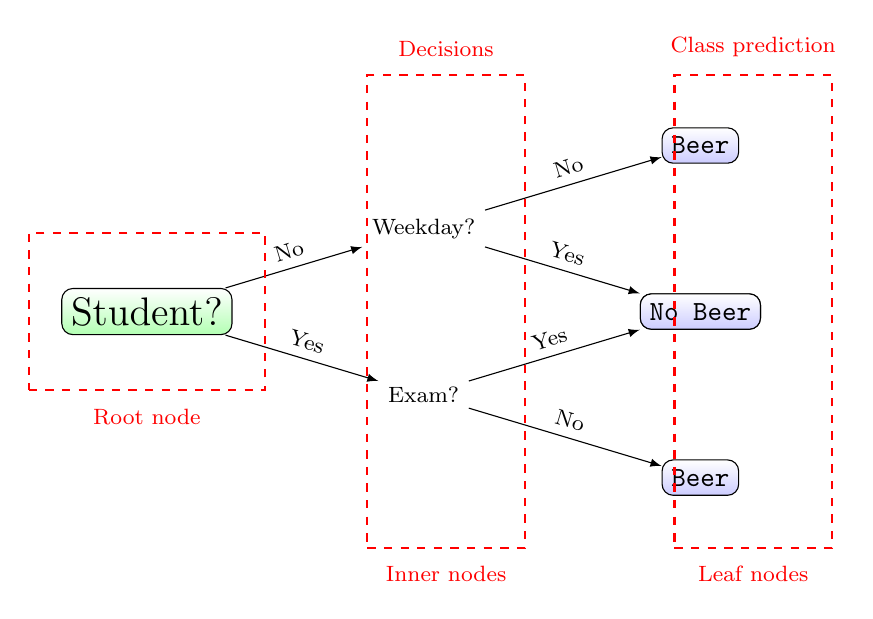
\begin{tikzpicture}
        [
            grow                    = right,
            sibling distance        = 6em,
            level distance          = 10em,
            edge from parent/.style = {draw, -latex},
            every node/.style       = {font=\footnotesize},
            sloped
        ]
	\node [root] {Student?}
        child { node [dummy] {Exam?}
                child { node [env] {Beer}
                        edge from parent node [above] {No} }
                child { node [env] {No Beer}
                        edge from parent node [above] {Yes} }                
                edge from parent node [above] {Yes} }
        child { node [dummy] {Weekday?}
                child { node [env] {No Beer}
                        edge from parent node [above] {Yes} }
                child { node [env] {Beer}
                        edge from parent node [above] {No} }                
                edge from parent node [above] {No} };
    \pause
    \node (rectroot) at (0,0) [rectangle, dashed, color=red, minimum height=2cm,minimum width=3cm,draw, thick] {};
    \node (rootbottom) [below=1mm of rectroot, color=red]  {Root node};
    \pause
    \node (rectinner) at (3.8,0) [rectangle, dashed, color=red, minimum height=6cm,minimum width=2cm,draw, thick] {};
    \node (innerbottom) [below=1mm of rectinner, color=red]  {Inner nodes};
    \node (innertop) [above=1mm of rectinner, color=red]  {Decisions};
    \pause
    \node (rectleaf) at (7.7,0) [rectangle, dashed, color=red, minimum height=6cm,minimum width=2cm,draw, thick] {};
    \node (leafbottom) [below=1mm of rectleaf, color=red]  {Leaf nodes};
    \node (leaftop) [above=1mm of rectleaf, color=red]  {Class prediction};

    \end{tikzpicture}
\end{frame}

%------------------------------------------------ 

\begin{frame}
    \frametitle{Decision tree learning}
    \vspace*{-7mm}
    \begin{block}{Training}
        \emph{Recursively} split feature space into sub-spaces at each step\\
        $\to$ Measures to evaluate split
        \begin{itemize}
            \item Error rate
            \item Information gain
            \item Gini index
        \end{itemize}
    \end{block}
\end{frame}

%------------------------------------------------ 

\subsection{Example}
\begin{frame}
    \frametitle{Decision tree learning}
    \centering\begin{tikzpicture}
        \node[inner sep=0pt] (featspace) at (0,0)
            {\includegraphics[height=3cm,keepaspectratio]{pics/DT-feature-space.png}};
        \node (featspaceTop) [above=1mm of featspace, color=black]  {Feature space};
        \node[inner sep=0pt] (nodes) at (3,-3.5)
            {\includegraphics[height=3.3cm,keepaspectratio]{pics/DT-fullygrown_nodes.png}};%
        \node (nodesTxt) [above=1mm of nodes, color=black]  {Decision tree};
        \node[inner sep=0pt] (DTapply) at (-3,-3.5)
            {\includegraphics[height=3.3cm,keepaspectratio]{pics/DT-fullygrown_feature_space.png}};
        \node (DTTxt) [above=1mm of DTapply, color=black]  {Classification};

        \draw[->,thick] (featspace.east) to [out=0,in=90] (nodesTxt.north) node[midway,above] {};
        \draw[->,thick] (featspace.west) to [out=180,in=90] (DTTxt.north) node[midway,above] {};
    \end{tikzpicture}
\end{frame}

%------------------------------------------------ 

\begin{frame}
    \frametitle{Decision tree learning}
    1) We compute a measure for \emph{each possible split} in each feature\\\hspace*{5mm}$\to$ here \textbf{absolute error rate} (AER)
    \\
    \vspace*{3mm}
    \centering\begin{tikzpicture}
        \node[inner sep=0pt, visible on=<1>] (feat1) at (0,0)
            {\includegraphics[height=4.5cm,keepaspectratio]{pics/DT-ER-y.png}};
        \node (feat1Txt) [above=1mm of feat1, color=black]  {\emph{y} split AER};
        % \node[inner sep=0pt, visible on=<2>] (feat2) at (0,0)
        %     {\includegraphics[height=4.5cm,keepaspectratio]{pics/DT-ER-x.png}};
        % \node (feat2Txt) [above=1mm of feat1, color=black,visible on=<2>]  {\emph{x}-\emph{y} split AER};
    \end{tikzpicture}
 
\end{frame}

%------------------------------------------------ 

\begin{frame}
    \frametitle{Decision tree learning}
    1) We compute a measure for \emph{each possible split} in each feature\\\hspace*{5mm}$\to$ here \textbf{absolute error rate} (AER)
    \\
    \vspace*{3mm}
    \centering\begin{tikzpicture}
        \node[inner sep=0pt] (feat2) at (0,0)
            {\includegraphics[height=4.5cm,keepaspectratio]{pics/DT-ER-x.png}};
        \node (feat2Txt) [above=1mm of feat1, color=black]  {\emph{x}-\emph{y} split AER};
        \pause
        \node (el) at (-0.53,-1.8) [ellipse, color=red, minimum height=5mm,minimum width=10mm,draw, ultra thick] {};
        \node (txt) at (3.5,-1.8) [color=red, ultra thick] {Minimum AER};
        \draw[->, color=red, ultra thick] (txt) to [out=160, in=20] (el);

    \end{tikzpicture}
 
\end{frame}

%------------------------------------------------ 

\begin{frame}
    \frametitle{Decision tree learning}
    1) We compute a measure for \emph{each possible split} in each feature\\\hspace*{5mm}$\to$ here \textbf{absolute error rate} (AER)\\
    2) Recursively repead step (1) for each subspace until AER $\to 0$
    \\
    \vspace*{3mm}
    \centering\includegraphics<1>[height=4.3cm,keepaspectratio]{pics/DT_1_split.png}%
    \centering\includegraphics<2>[height=4.6cm,keepaspectratio]{pics/DT_2_split.png}%
    \centering\includegraphics<3>[height=4.6cm,keepaspectratio]{pics/DT_3_split.png}%
    \centering\includegraphics<4>[height=4.6cm,keepaspectratio]{pics/DT_4_split.png}%
    \centering\includegraphics<5>[height=4.6cm,keepaspectratio]{pics/DT_5_split.png}%
    \centering\includegraphics<6>[height=4.3cm,keepaspectratio]{pics/DT_final.png}%
     
\end{frame}

%------------------------------------------------ 

\begin{frame}
    \frametitle{Decision tree classification}
    3) Classification
    \\
    \vspace*{3mm}
    \includegraphics[height=4.3cm,keepaspectratio]{pics/DT_classification.png}%
 
\end{frame}

%------------------------------------------------ 

\begin{frame}
    \frametitle{Decision tree improvements I}
    \begin{itemize}
        \item Use more sophisticated split measures 
            \begin{itemize}
                \item \emph{Information gain} $\leftrightarrow$ (im-)purity of splitted sub-sets
                \item Gini index
            \end{itemize}
        \item Pruning 
    \end{itemize}
    \vspace*{3mm}
    \centering\begin{tikzpicture}
        \node[inner sep=0pt] (IG) at (3,0)
            {\includegraphics[height=3.5cm,keepaspectratio]{pics/DT_info-gain.png}};
        \node (IGtxt) [below=1mm of IG, color=black]  {Information gain};
        \node[inner sep=0pt] (AER) at (-3,0)
            {\includegraphics[height=3.5cm,keepaspectratio]{pics/DT_AER.png}};
        \node (AERtxt) [below=1mm of AER, color=black]  {Absolute error rate};
        \draw[->, color=red, ultra thick] (AER) to [out=0, in=180] (IG);
    \end{tikzpicture}
 
\end{frame}

%------------------------------------------------ 

\subsection{Improvements}
\begin{frame}
    \frametitle{Decision tree improvements II}
    \begin{columns}[T] % align columns        
        \begin{column}{.48\textwidth}
            \begin{block}{Random forest}
                \begin{itemize}
                    \item<1-> Ensemble of DTs
                    \item<2-> For each tree use:
                    \begin{itemize}
                        \item<3-> Random sub-sample (=\emph{bootstrapping})
                        \item<4-> Random number of the original features\\
                                  $\to$ large number of rather shallow trees
                    \end{itemize}
                    \item<5-> Classify data by majority voting of individual trees
                \end{itemize}
            \end{block}
        \end{column}%
        \hfill%
        \begin{column}{.48\textwidth}
            \begin{block}{Boosted DT}
                \begin{itemize}
                    \item<6-> Sequential ensemble of evolving DTs
                    \item<7-> Output of each tree is given weight relative to accuracy
                    \item<8-> $\to$ Subsequent predictors learn from the mistakes of the previous predictors
                \end{itemize}
            \end{block}            
        \end{column}%
    \end{columns}

\end{frame}

%------------------------------------------------ 

\section{Linear cuts}

\begin{frame}
    \frametitle{Linear cuts}
    \begin{columns}[T] % align columns        
        \begin{column}{.48\textwidth}
            % \color{red}\rule{\linewidth}{4pt}
            More flexible than rectangular cut
            \begin{itemize}
                \item<1-> Simple white box methods 
                \item<2-> Can become very powerful by using \emph{kernel trick}
            \end{itemize}
        \end{column}%
        \hfill%
        \begin{column}{.48\textwidth}
            % \color{blue}\rule{\linewidth}{4pt}
            % \hspace*{-10mm}
            \raggedright\includegraphics[height=4.3cm,keepaspectratio]{pics/mva_cut_linear.png}%
            
        \end{column}%
    \end{columns}

\end{frame} 

%------------------------------------------------ 





\end{document}

